\chapter{Thực nghiệm}
Để có cái nhìn tổng quan về các phương pháp đã đề cập đến ở chương trước, nhóm báo cáo đã tiến hành tổng hợp bộ dữ liệu được sử dụng của mỗi phương pháp và tổng hợp kết quả so sánh được đề cập trong mỗi phương pháp. Chương này trình bày bảng tổng hợp bộ dữ liệu, xây dựng bộ dữ liệu chung, sử dụng bộ dữ liệu chung để tiến hành các thực nghiệm trên 3 phương pháp là PHACTS, Phage AI và DeePhage. Cuối cùng, nhóm báo cáo sẽ trình bày kết quả thực nghiệm và phân tích kết quả.

\section{Tổng hợp bộ dữ liệu}
Các bộ dữ liệu được đề cập đến trong các phương pháp bao gồm:
\begin{itemize}
    \item PHACTS: Nhóm tác giả PHACTS đã sử dụng bộ dữ liệu PHANTOME. Trong bộ dữ liệu PHANTOME có 654 bộ gen thực khuẩn. Tuy nhiên, nhóm tác giả PHACTS đã lựa chọn thủ công và chỉ sử dụng 227 dữ liệu. Trong đó bao gồm 148 bộ gen thực khuẩn thể ôn hoà và 79 bộ gen thực khuẩn thể độc lực. Tỉ lệ nhãn trong bộ dữ liệu này là 2:1. Bộ dữ liệu này cũng được đề cập và sử dụng lại ở các phương pháp khác là DeePhage, PhaTYP và PhageBERT.
    \item ACLAME và PhagesDB: Nhóm tác giả PhageAI đã sử dụng hai bộ dữ liệu này để huấn luyện mô hình phân loại thực khuẩn. Trong bài báo, nhóm tác giả không mô tả chi tiết về số lượng dữ liệu cũng như cách chọn dữ liệu từ hai tập dữ liệu này. Nhóm tác giả chỉnh sửa thủ công và chọn ra bộ dữ liệu huấn luyện gồm: 278 bộ gen thực khuẩn thể độc lực và 174 bộ gen thực khuẩn thể ôn hoà. Và bộ dữ liệu thử nghiệm gồm 54 bộ gen thực khuẩn thể độc lực và 30 bộ gen thực khuẩn thể ôn hoà. Tổng cả có thể xem bộ dữ liệu này gồm 536 bộ gen thực khuẩn.
    \item Mavrich \& Hatfull (2017): Bộ dữ liệu này được giới thiệu ở bài báo của Mavrich \& Hatfull (2017). Bộ dữ liệu này gồm 1057 bộ gen thực khuẩn. 
    \item NCBI-tháng 3 năm 2021: Bộ dữ liệu này gồm 1640 bộ gen thực khuẩn. Trong đó, 1211 bộ gen thực khuẩn thể độc lực và 429 bộ gen thực khuẩn thể ôn hoà. 
    \item NCBI RefSeq 2022: Bộ dữ liệu này gồm 3474 bộ gen thực khuẩn được công bố trước năm 2022. Bộ dữ liệu này được PhaTYP sử dụng cho nhiệm vụ học tự giám sát và nhiệm vụ tinh chỉnh. Trong đó, nhiệm vụ học tự giám sát sử dụng 3474 bộ gen thực khuẩn. Nhiệm vụ tinh chỉnh sử dụng 1290 thực khuẩn thể độc lực và 577 thực khuẩn thể ôn hoà.
    \item NCBI- tháng 10 năm 2024: Nhóm tác giả của DeepPL sử dụng cơ sở dữ liệu NCBI với các cập nhật mới hơn bản tháng 3 năm 2021. Nhóm tác giả DeepPL sử dụng bộ dữ liệu huấn luyện gồm 1262 bộ gen thực khuẩn thể độc lực và 557 bộ gen thực khuẩn thể ôn hoà. Tập dữ liệu kiểm thử gồm 245 bộ gen thực khuẩn thể độc lực và 129 bộ gen thực khuẩn thể ôn hoà. 
\end{itemize}

Các bộ dữ liệu trên được sử dụng ở các phương pháp như sau:
\begin{table}[H]
    \centering
    \begin{tabular}{|m{5cm}|m{5cm}|>{\raggedleft\arraybackslash}m{3cm}|}
        \hline
        Tên phương pháp & Bộ dữ liệu & Tổng số\\
        \hline
        PHACTS & PHACTS & 227\\
        \hline
        PhageAI & ACLAME và PhagesDB & 536\\
        \hline
        BACPHLIP & Mavrich \& Hatfull (2017) & 1057 \\ 
        \hline
        DeePhage & PHACTS và NCBI- tháng 3 năm 2021 & 1867 \\
        \hline
        PhaTYP - nhiệm vụ học tự giám sát & NCBI RefSeq 2022 & 3474 \\
        \hline
        PhaTYP - nhiệm vụ tinh chỉnh & NCBI RefSeq 2022 & 1867 \\
        \hline
        DeepPL & NCBI- tháng 10 năm 2024 & 2193 \\
        \hline
    \end{tabular}
    \caption{Tổng hợp bộ dữ liệu của các phương pháp đã đề cập}
    \label{tab:dataset_summary}
\end{table}

Từ kết quả tổng hợp ở bảng \ref{tab:dataset_summary}, nhóm báo cáo rút ra một số nhận xét như sau:

Thứ nhất, các phương pháp giới thiệu sau có xu hướng sử dụng bộ dữ liệu lớn hơn so với các phương pháp trước đó. Điều này cho thấy rằng, các phương pháp sau đã có sự cải tiến trong việc thu thập và xử lý dữ liệu đầu vào. 

Thứ hai, các phương pháp sử dụng bộ dữ liệu khác nhau. Điều này dẫn đến việc không thể so sánh trực tiếp hiệu suất của các phương pháp với nhau.

Thứ ba, các phương pháp sau khi đưa ra so sánh hiệu suất với các phương pháp trước đó lại có kết quả công bố không đồng nhất. Ví dụ: trong phương pháp PHACTS, nhóm tác giả đã công bố độ chính xác là 98\% trên bộ dữ liệu PHACTS. Tuy nhiên, trong phương pháp BACPHLIP, nhóm tác giả BACPHLIP đã công bố độ chính xác của phương pháp PHACTS chỉ là 79\% trên tập dữ liệu Mavrich \& Hatfull (2017).

Từ những lí do trên, nhóm báo cáo đã quyết định xây dựng bộ dữ liệu thống nhất và thực hiện các thực nghiệm chung trên cùng bộ dữ liệu để đưa ra kết quả so sánh chính xác hơn giữa các phương pháp. 


\section{Xây dựng bộ dữ liệu}
\subsection{ Xử lý nhãn }
Sau khi tìm hiểu các bài báo, nhóm báo cáo thực hiện xây dựng bộ dữ liệu mới dựa trên 2 bộ dữ liệu được sử dụng trong bài báo DeepPL và DeePhage. Nhãn $y$ của bản ghi $X$ được nhóm báo cáo xử lý như sau:
\begin{enumerate}
    \item Nếu $X \in DeePhage \Rightarrow y = y_{DeePhage}$ 
    \item Nếu $X \in DeepPL \Rightarrow y = y_{DeepPL}$
    \item Nếu $X \in DeePhage \cap DeepPL \Rightarrow y = y_{DeePhage}$
\end{enumerate}

\section{Kịch bản thực nghiệm}\label{ kịch bản thực nghiệm}
Để tiến hành các thực nghiệm, nhóm báo cáo chọn 2 mô hình là DeePhage và XGBoost. Nhận thấy DeePhage là công cụ  hài hòa trong nhóm các phương pháp dựa trên học sâu khi mà hiệu suất phân loại tốt đồng thời có thời gian huấn luyện nhanh, nhóm báo cáo quyết định chọn DeePhage là công cụ tiêu chuẩn trong các thực nghiệm. Ngoài ra, do cần 1 mô hình đủ mạnh để có thể có hiệu suất phân loại tốt cũng như nhanh trong quá trình huấn luyện, nhóm quyết định chọn XGBoost là mô hình được sử dụng để trực tiếp so sánh với DeePhage.

\section{Các chỉ số đánh giá}
Để đánh giá 1 cách toàn diện hiệu suất phân loại của mô hình chứ không chỉ tập trung vào nhãn 1, nhóm báo cáo sử dụng các chỉ số sau:
\begin{itemize}
    \item Accuracy: sử dụng để do lường hiệu suất phân loại chung của mô hình trên 2 nhãn.
    \item Sensitivity: sử dụng để đo lường dộ phủ của mô hình trên nhãn 1.
    \item Specificity: sử dụng để đo lường độ phủ của mô hình trên nhãn 0.
\end{itemize}

\section{Kết quả}
\subsection{Thực nghiệm với mô hình PHACTS}
Để tiến hành thực nghiệm với mô hình PHACTS, nhóm báo cáo đã sử dụng bộ mã nguồn của mô hình PHACTS được nhóm tác giả công bố trên Github tại địa chỉ: \url{https://github.com/deprekate/PHACTS} (truy cập ngày 23 tháng 5 năm 2025). Quá trình thực hiện các thực nghiệm có các bước như sau:
\begin{itemize}
    \item \textbf{Xử lí đữ liệu} Bộ dữ liệu chung của nhóm báo cáo chứa thông tin DNA, trong khi PHACTS yêu cầu đầu vào là dữ liêu protein. Do đó, nhóm báo cáo thực hiện chuyển đổi bộ dữ liệu đầu vào từ DNA sang protein. 
    \item \textbf{Huấn luyện mô hình} Bộ dữ liệu huấn luyện được sử dụng là bộ dữ liệu được nhóm báo cáo xây dựng. Bộ dữ liệu gồm 1733 bộ gen thực khuẩn. Trong đó, 1184 bộ gen thực khuẩn thể độc lực và 549 bộ gen thực khuẩn thể ôn hoà. 
    \item \textbf{Đánh giá mô hình} Nhóm báo cáo sử dụng bộ dữ liệu thử nghiệm là bộ dữ liệu được nhóm báo cáo xây dựng. Bộ dữ liệu gồm 434 bộ gen thực khuẩn. Trong đó, 296 bộ gen thực khuẩn thể độc lực và 138 bộ gen thực khuẩn thể ôn hoà.
    \item \textbf{Thu thập kết quả} Để có kết quả sát thực với thực tế, nhóm báo cáo đã tiến hành chạy thử nghiệm 10 lần. Mỗi lần chạy thử nghiệm nhóm báo cáo thu thập các chỉ số đánh giá là Accuracy, Sensitivity và Specificity. Nhóm báo cáo đã tính toán trung bình cộng của 10 lần chạy thử nghiệm để có kết quả cuối cùng. Kết quả cuối cùng được nhóm báo cáo trình bày trong bảng \ref{tab:result_phacts}.
\end{itemize}


\begin{table}[H]
    \centering
    \begin{tabular}{|m{5cm}|m{5cm}|>{\raggedleft\arraybackslash}m{3cm}|}
        \hline
        Chỉ số & Giá trị & Độ lệch chuẩn\\
        \hline
        Accuracy & 0.712442 & 0.016727\\
        \hline
        Sensitivity & 0.827703 & 0.022537\\
        \hline
        Specificity & 0.465217 & 0.032163\\ 
        \hline
    \end{tabular}
    \caption{Kết quả thực nghiệm với mô hình PHACTS}
    \label{tab:result_phacts}
\end{table}

Nhóm báo cáo nhận thấy rằng, với bộ dữ liệu dùng chung ở trên, mô hình PHACTS cho kết quả Accuracy là 71.24\%, Sensitivity là 82.77\% và Specificity là 46.52\%. Kết quả này thấp hơn nhiều so với kết quả công bố của nhóm tác giả PHACTS (đã đề cập ở phần trước).





\subsection{Kết quả thực nghiệm với PhageAI}
Trong thí nghiệm này, chúng tôi thực hiện thử nghiệm các thuật toán học máy trong bài báo PhageAI với bộ dữ liệu mới. Các mô hình đều sử dụng BayesianSearch để tối ưu lựa chọn các bộ tham số tốt nhất. Riêng với thuật toán SVM, chúng tôi sử dụng bộ tham số đã được tác giả công bố trong bài báo.
\begin{table}[ht]
\footnotesize
\centering
\begin{tabular}{|l|c|c|c|}
\hline
\textbf{Model} & \textbf{Accuracy} & \textbf{Sensitivity (Class 1)} & \textbf{Specificity (Class 0)} \\
\hline
GaussianNB & 0.649 & 0.780 & 0.365 \\
SGDClassifier & 0.864 & 0.861 & 0.869 \\
MLPClassifier & 0.901 & 0.946 & 0.803 \\
RandomForestClassifier & 0.928 & \textbf{0.963} & 0.854 \\
SVC & 0.901 & 0.882 & \textbf{0.942} \\
KNeighborsClassifier & 0.910 & 0.909 & 0.912 \\
GradientBoostingClassifier & 0.930 & 0.951 & 0.882 \\
XGBoost & \textbf{0.936} & 0.959 & 0.883 \\
LightGBM & 0.933 & 0.951 & 0.878 \\
CatBoost & 0.931 & 0.953 & 0.870 \\
\hline
\end{tabular}
\caption{Kết quả so sánh các thuật toán học máy theo Accuracy, Sensitivity và Specificity trên bộ dữ liệu kết hợp.}
\label{tab:model_comparison}
\end{table}

Dựa trên kết quả Bảng \ref{tab:model_comparison}, có thể thấy rằng các mô hình thuộc nhóm ensemble learning, đặc biệt là các thuật toán Boosting như XGBoost, LightGBM, CatBoost và GradientBoostingClassifier, đều cho hiệu suất rất cao trên cả ba chỉ số: Accuracy, Sensitivity và Specificity. Trong đó, XGBoost đạt Accuracy cao nhất (0.936), đồng thời duy trì mức Sensitivity (0.959) và Specificity (0.883) rất cân bằng, cho thấy khả năng phân biệt tốt giữa hai lớp.

RandomForestClassifier cũng thể hiện hiệu quả cao với Accuracy 0.928, tuy nhiên có phần thiên lệch hơn về Sensitivity (0.963) so với Specificity (0.854), nghĩa là mô hình có xu hướng nhạy hơn với lớp dương (Class 1).

Ở nhóm mô hình cơ bản hơn như GaussianNB và SGDClassifier, kết quả không thực sự khả quan. Đặc biệt, GaussianNB cho Specificity chỉ ở mức 0.365, cho thấy mô hình này khó phân biệt được lớp âm (Class 0), mặc dù có Sensitivity tương đối tốt (0.780). Điều này thường xảy ra khi dữ liệu không phù hợp với giả định phân phối chuẩn của Naive Bayes.

MLPClassifier và SVC đều có Accuracy trên 0.9, nhưng mỗi mô hình có thiên hướng riêng: MLPClassifier nghiêng về phát hiện Class 1 (Sensitivity cao 0.946), trong khi SVC lại rất mạnh trong việc nhận diện Class 0 (Specificity 0.942).

Tổng thể, như vậy khác với tập dữ liệu của bài báo với SVC cho kết quả tốt nhất thì trong thực nghiệm này, các mô hình Boosting như XGBoost và GradientBoostingClassifier tỏ ra vượt trội về độ chính xác và cân bằng giữa các chỉ số, phù hợp với các bài toán phân loại nhị phân có yêu cầu cao về độ tin cậy. 


\subsection{Thực nghiệm với mô hình DeePhage}
<<Sơn điền kết quả>>

\section{So sánh kết quả thực nghiệm giữa các mô hình}


\subsection{So sánh hiệu suất phân loại giữa DeePhage và XGBoost trên bộ dữ liệu xây dựng}

\begin{figure}[H]
    \centering
    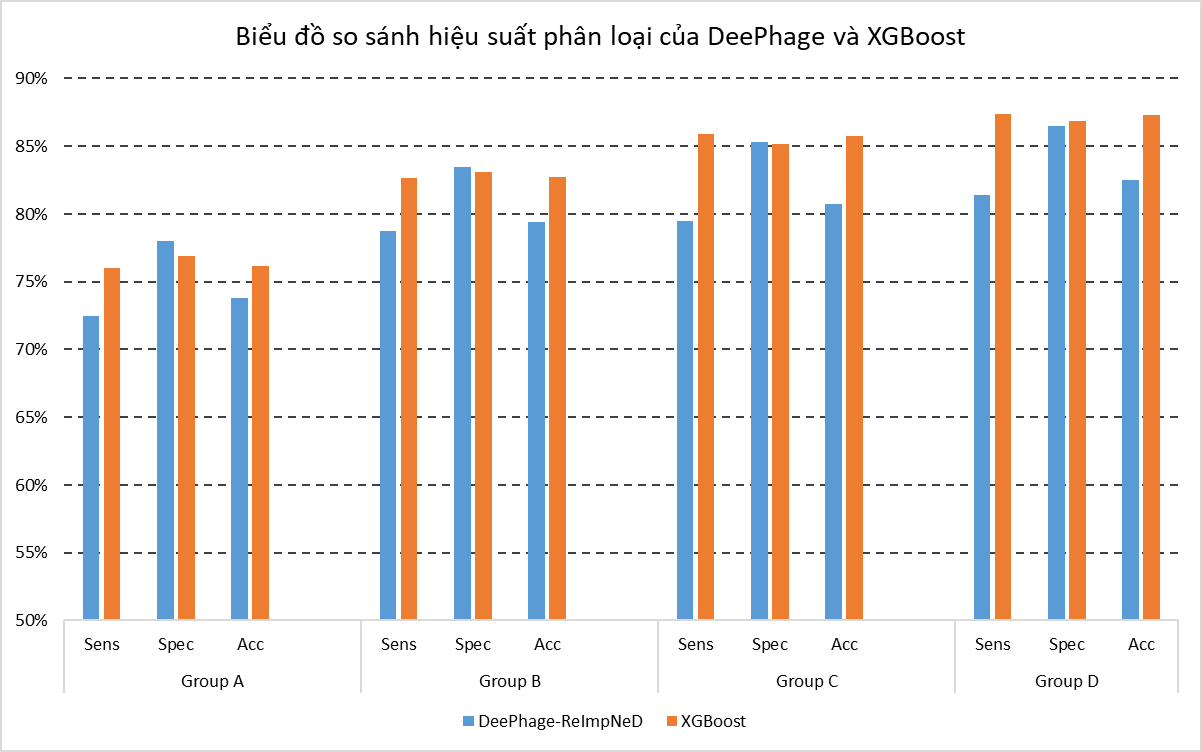
\includegraphics[width=1\linewidth]{figures/result_deephage_vs_xgboost.png}
    \caption{Kết quả hiệu suất phân loại của mô hình XGBoost trên tập dữ liệu xây dựng.}
    \label{fig:result_2}
\end{figure}

Hình \ref{fig:result_2} là biểu đồ so sánh hiệu suất phân loại của DeePhage và XGBoost trên tập dữ liệu mà nhóm báo cáo xây dựng. Có thể thấy, DeePhage cho kết quả tốt hơn 1 chút, khoảng từ 2\% - 5\% khi hơn XGBoost ở 2 chỉ số Sensitivity và Accuracy. Nghĩa là DeePhage cho khả năng nhận diện nhãn 1 và độ chính xác tổng thể cao hơn. Với chỉ số Specificity, XGBoost cho kết quả tốt hơn khoảng 5\%, nghĩa là khả năng nhận diễn nhãn 0 của XGBoost tốt hơn DeePhage.

